\documentclass[11pt]{article}
\usepackage[T1]{fontenc}
\usepackage[utf8]{inputenc}
\usepackage{lmodern,microtype}
\usepackage[margin=1in,headheight=15pt]{geometry}
\usepackage{amsmath,amssymb,amsthm,mathtools}
\usepackage{booktabs,longtable,array,enumitem,graphicx,xcolor}
\usepackage{fancyhdr}
\usepackage[colorlinks=true,linkcolor=blue!45!black,citecolor=blue!45!black,urlcolor=blue!45!black]{hyperref}
\usepackage{xurl}
\hypersetup{pdftitle={Beyond Dirichlet GRH: validated arithmetic and transferable proof machinery},pdfauthor={Research report prepared for Vladimir Reshetnikov}}
\definecolor{ink}{HTML}{19384A}
\definecolor{accent}{HTML}{1C746D}
\pagestyle{fancy}
\fancyhf{}
\fancyhead[L]{\small Beyond Dirichlet GRH}
\fancyhead[R]{\small Research synthesis}
\fancyfoot[C]{\thepage}
\setlength{\parindent}{0pt}
\setlength{\parskip}{5pt plus 1pt}
\setlength{\emergencystretch}{3em}
\setlist{itemsep=3pt,topsep=4pt}
\newtheorem{theorem}{Theorem}[section]
\newtheorem{proposition}[theorem]{Proposition}
\newtheorem{lemma}[theorem]{Lemma}
\newtheorem{corollary}[theorem]{Corollary}
\theoremstyle{remark}
\newtheorem{remark}[theorem]{Remark}
\newcommand{\R}{\mathbb R}
\newcommand{\C}{\mathbb C}
\newcommand{\Q}{\mathbb Q}
\newcommand{\N}{\mathbb N}
\newcommand{\Z}{\mathbb Z}
\newcommand{\Gal}{\operatorname{Gal}}
\newcommand{\Tr}{\operatorname{Tr}}
\newcommand{\pos}[1]{\left(#1\right)_{+}}
\newcommand{\src}[2]{\href{https://github.com/lsernau/grh-lean/blob/72fead102f663d5c7a407964a13dc0cf9d977207/grh/src/#1.lean}{\nolinkurl{#2}}}
\newcommand{\priorurl}{https://github.com/VladimirReshetnikov/ProveIt/tree/6fe2c1bd450aa7f19eab17fb9a6e76170b4fce00/docs/incoming}
\begin{document}
\begin{titlepage}
\vspace*{1.0cm}
{\small\sffamily\color{accent} RESEARCH REPORT\par}
\vspace{0.6cm}
{\fontsize{29}{35}\selectfont\bfseries\color{ink} Beyond Dirichlet GRH\par}
\vspace{0.35cm}
{\Large Validated arithmetic and transferable proof machinery\par}
\vspace{0.6cm}
{\large Prepared for Vladimir Reshetnikov\par}
{25 November 2026 (Pacific time)\par}
\vspace{0.8cm}
\textbf{Main finding.} The supplied research already contains an arithmetic completion that goes beyond a previously known GRH implication: the exponent-six imaginary quadratic class-group census. Its proof has been reviewed and both complete finite searches replayed here. Exactly 432 fields occur. The published census below $3.1\cdot10^{20}$ remains an explicitly cited input.

\textbf{Further method transfer.} An explicit integral frame over a real nonabelian $S_3$ field realizes a local ingredient of the theta-derivative machinery. Two analytic interfaces are developed: joint positive averages with no common spectral zeros, and sharp conversion of positive-ramp moment bounds to pointwise bounds. These are proved downstream statements; they do not establish nonabelian GRH.

\textbf{Scope of verification.} This report pins and inspects the Lean source, reviews all 26 incoming GRH archives, reruns exact arithmetic certificates, and compiles seven elementary Lean lemmas. It does not claim to have rebuilt the complete upstream development or formalized the downstream analysis end to end.
\vfill
\small
Source: \nolinkurl{lsernau/grh-lean}, commit \texttt{72fead102f663d5c7a407964a13dc0cf9d977207}.\\
Prior reports: \nolinkurl{VladimirReshetnikov/ProveIt}, commit \texttt{6fe2c1bd450aa7f19eab17fb9a6e76170b4fce00}.\\
Full proofs, exact checkers, validation logs, source map, prior-work matrix, and dependency pins accompany this PDF.
\end{titlepage}
\tableofcontents
\newpage
\section{Answer and evidence boundary}

There are useful transfers beyond familiar consequences of RH and Dirichlet GRH. The strongest conclusion supported by this investigation has two parts. First, a previous ProveIt report contains a complete extra arithmetic argument for a classification that was still conditional on an unsearched interval in the cited literature. Its decisive certificates reproduce successfully. Second, the internal proof machinery has genuinely reusable pieces, but the passage to a new nonabelian zero theorem still requires an arithmetic comparison not supplied by the repository or by the incoming reports.

\subsection{A result that can be endorsed now}

The exponent-six completion in \emph{grh-exponent-six-and-transfers.zip} proves that exactly 432 imaginary quadratic fields have ideal class group of exponent six. Aiken--Ross--Shvydkoy--Xue's Theorem 1.3(5) still leaves a fundamental-discriminant interval to exclude even under ERH. The previous report eliminates that interval by an explicit-formula test, a collision between two integral norm equations, and an exact residue sieve. Here its mathematical reduction was reviewed, its interval-arithmetic test rerun, and both independent complete divisor searches reproduced. This is a validation and re-exposition of earlier work, not a claim of discovering the classification during the present turn.\cite{priorSix,EKN,ARSX}

The extension from fields to orders then gives 1,236 orders of exact exponent six. The field list and the order-table identity were checked. The underlying published exhaustive enumeration through $3.1\cdot10^{20}$ was not rerun; it is used as a published computational theorem. Section~\ref{sec:census} makes all dependencies explicit.

This application uses the exported quadratic-GRH theorem together with a substantial additional argument. It differs from importing a ready-made conditional consequence, and it also differs from directly transplanting the source's unitary theta-lift construction. Both distinctions matter to the requested scope.

\subsection{New work in this synthesis}

The following additions were not found in the 26 inspected archives. Their mathematical ingredients have classical antecedents, so no claim of worldwide priority is made.
\begin{enumerate}
\item An explicit trace frame over the real $S_3$ splitting field of $T^3-4T+1$, together with a cyclotomic tensor construction and a precise local Frobenius compatibility. This realizes one local input for a nonabelian extension; it is more concrete than merely specifying a desired prime statistic.
\item A joint positive-averaging criterion: several individually imperfect averages detect every pole if their Mellin multipliers have no common zero. An integer-coefficient two-filter example comes with an exact polynomial identity and a sharp obstruction when a common zero exists.
\item A positive-ramp $L^p$-to-pointwise estimate with optimal exponent, including a countermodel with uniformly bounded positive real coefficients supported on the integers. It explains why direct averaged Landau arguments are valuable: one should not insist on recovering the full pointwise error first.
\end{enumerate}

\subsection{What the source proves}

The public endpoints in \src{Statements}{Statements.lean} and \src{Main}{Main.lean} concern the Riemann zeta function and Dirichlet characters over $\Q$. In particular, the theorem \texttt{LFunction\_eq\_zero\_re} states that a Dirichlet $L$-function zero in $0<\Re s<1$ has real part $1/2$. It does not quantify over all Hecke characters of all number fields, all Artin representations, or all automorphic representations.\cite{source}

Independent public checks report successful compilation and axiom checks of both shortened editions; the compact project also has a reported complete Lean kernel replay. These external reports support taking the supplied theorem as the starting point. The source examination in this session is not an independent rerun of those complete checks.\cite{Sutherland,Rubinstein}

\subsection{A baseline that avoids repeated reductions}

The earlier reports already develop precise nonabelian detectors for cubic and quintic fields, $S_n$, $A_5$, $A_6$, Sylow subgroups, cyclic generators, reflection groups, and $\operatorname{PSL}_2$. They also contain reciprocal convexity, fourth-power sampling, positive-part Mellin criteria, moving-box averages, torsion selection, and ramification-aware Selmer warnings. Appendix~A and the accompanying claim matrix record all 26 packages.\cite{priorCollection}

The fourth-power sampling idea is therefore explicitly credited to the prior reports and their cited antecedent, rather than counted as new. Likewise the positive-part Mellin lemma below is reused from the previous mean-transfer report. The contribution of the present analytic sections is the joint-filter repair and the sharp positive-ramp specialization.\cite{priorSampling,priorMean,Setiawan}

\section{A completed arithmetic application: exponent six}
\label{sec:census}

This section re-exposes and validates the proof in the earlier exponent-six report. The new work here is the independent review and complete replay of its decisive finite tests.\cite{priorSix}

\begin{theorem}[Completion of the exponent-six census]
There are exactly 432 imaginary quadratic number fields whose ideal class group has exact exponent six. The largest absolute fundamental discriminant among them is $5\,761\,140$. There are exactly 1,236 imaginary quadratic orders of exact class-group exponent six, with largest absolute discriminant $43\,522\,752$.
\end{theorem}

The group exponent is the least positive integer killing every ideal class. The proof uses Dirichlet GRH as supplied by the Lean source. It also uses two published inputs: the exhaustive field census through
\[
 X_0=3.1\cdot10^{20},
\]
and the quadratic-GRH upper bound
\[
 |D|\le X_1=2.5\cdot10^{25}
\]
for exponent-six fields. Both are in Elsenhans--Kl\"uners--Nicolae (EKN). Their original ERH completeness theorem excludes exponent six; the interval $(X_0,X_1]$ requires the extra argument below. The order assertion then uses the conductor classification of Aiken--Ross--Shvydkoy--Xue.\cite{EKN,ARSX}

\subsection{Integral norms constrain every small split prime}

Suppose that $D<0$ is fundamental, $x=|D|>X_0$, and the class group is killed by six. If a rational prime $p$ splits, write $p\mathcal O_K=\mathfrak p\overline{\mathfrak p}$. Then $\mathfrak p^6$ is principal, generated by an algebraic integer of the form $(a+b\sqrt D)/2$. The coefficient $b$ is nonzero: a rational generator would have equal valuations at the two conjugate prime ideals. Taking absolute values of the coefficients yields
\begin{equation}\label{eq:norm6}
 a_p^2+x b_p^2=4p^6,\qquad a_p\ge0,\quad b_p\ge1.
\end{equation}
In particular $x\le4p^6$. Since $4\cdot2000^6<X_0$, every split prime in a putative omitted field exceeds 2000.

\subsection{A signed test with nonnegative Fourier transform}

Let $Y=5500$, $\delta=\log Y/12$, and let $g$ take the following values on successive intervals of length $\delta$, starting at zero, and vanish elsewhere:
\[
 21,14,10,6,4,1,-1,-4,-6,-10,-14,-21.
\]
Define its normalized autocorrelation and Fourier transform by
\[
 F(u)=\frac{\int_\R g(v)g(v+u)\,dv}{\int_\R g(v)^2\,dv},
 \qquad h(t)=\int_\R F(u)e^{itu}\,du.
\]
The function $F$ is even, piecewise linear, supported on $[-\log Y,\log Y]$, and satisfies $F(0)=1$, $|F|\le1$. Its transform $h$ is nonnegative on $\R$, because it is a squared Fourier modulus divided by $\|g\|_2^2$. The step-function construction also makes $h$ entire with quadratic decay on each fixed horizontal strip.

For the primitive odd quadratic character $\chi(n)=(D/n)$, the Guinand--Weil formula in this normalization is
\begin{align}
 \sum_\rho h\bigl((\rho-1/2)/i\bigr)
 ={}&\log(x/\pi)
 +\frac1{2\pi}\int_\R h(t)\Re\frac{\Gamma'}\Gamma(3/4+it/2)\,dt\notag\\
 &-2\sum_{n\ge2}\frac{\chi(n)\Lambda(n)}{\sqrt n}F(\log n).
 \label{eq:explicit6}
\end{align}
The supplied quadratic GRH makes the left side nonnegative. The analytic identity and its test-function hypotheses are standard; the cited Fourier-optimization paper states a compatible version as Lemma 9.\cite{Carneiro}

Write $C$ for the maximum absolute slope of $F$, and $\psi=\Gamma'/\Gamma$. Fourier inversion and the integral formula for $\psi$ give
\[
 \frac1{2\pi}\int_\R h(t)\Re\psi(3/4+it/2)\,dt
 =\psi(3/4)+2\int_0^\infty
   \frac{e^{-3u/2}}{1-e^{-2u}}(1-F(u))\,du
 \le\psi(3/4)+\frac{14}9 C.
\]
Indeed $0\le1-F(u)\le Cu$, and
\[
 \sum_{j\ge0}(2j+3/2)^{-2}\le\frac49+\frac13=\frac79.
\]
The elementary bound $\log\pi-\psi(3/4)>2$ follows from
$\log\pi>1.1$, $\gamma>1/2$, and
$\psi(1)-\psi(3/4)>1/3+1/14$. Therefore
\begin{equation}\label{eq:prime-test6}
 \log x>
 2\sum_{n\ge2}\frac{\chi(n)\Lambda(n)}{\sqrt n}F(\log n)
 +2-\frac{14}9 C.
\end{equation}

The signed values of $g$ are significant. Although $h$ is nonnegative, $F$ can be negative near the end of its support. An inert prime, for which $\chi(p)=-1$, can then contribute positively to the right side. This combines a positive spectral test with an arithmetic exclusion pattern.

\subsection{At least 28 split primes, but at most 18 coefficients}

Use the all-inert model
\[
 R_p=2\sum_{p^k\le Y}\frac{(-1)^k}{\sqrt{p^k}}F(k\log p),
 \quad S=\sum_{p\le Y}R_p\log p,
 \quad B=\max(0,\max_{p\le Y}R_p).
\]
Removing a ramified prime loses at most $R_p\log p$, so the total loss is at most $B\log x$. Every split prime exceeds 2000, and its square exceeds $Y$; changing it from inert to split loses
\[
 L_p=-4\frac{\log p}{\sqrt p}F(\log p).
\]
If $N_Y$ split primes occur below $Y$, and $L$ bounds all these losses from above, \eqref{eq:prime-test6} implies
\[
 N_Y L>S+2-\frac{14}9C-(1+B)\log X_1.
\]
The accompanying rational checker proves, with strict enclosures,
\begin{equation}\label{eq:exact-margins}
 \max_{2000<p\le5500}L_p<0.216,
 \qquad S+2-\frac{14}9C-(1+B)\log X_1>5.84.
\end{equation}
Because $27\cdot0.216=5.832<5.84$, one obtains $N_Y\ge28$.

On the other hand, \eqref{eq:norm6} and
\[
 4\cdot5500^6<19^2X_0
\]
give $1\le b_p\le18$. Two distinct split primes $p<q$ must therefore share the same $b$.

The checker obtains rigorous logarithm bounds from the positive series for $2\operatorname{arctanh}z$, after range reduction to $1\le u\le2$, with a rational geometric tail. Square-root bounds use integer square roots. The knot containing $\log(p^k)$ is located by comparing $(p^k)^{12}$ with powers of $Y$. No floating-point sign decision enters \eqref{eq:exact-margins}.

\subsection{A finite certificate eliminates the collision}

For two equations with the same $b$, set $A=a_p$, $A'=a_q$. Their squares differ by a multiple of four, so $A,A'$ have the same parity. Put
\[
 u=(A'-A)/2,\quad v=(A'+A)/2,\quad
 N=q^6-p^6=uv.
\]
Here $0<u\le v$, $A=v-u$, and
\begin{equation}\label{eq:candidate6}
 M=4p^6-(v-u)^2=x b^2>X_0.
\end{equation}
For a divisor $u\mid N$ with $u\le\sqrt N$, positivity of $M$ is equivalent to $u>q^3-p^3$. Hence the search is finite:
\[
 p<q\le5500,\quad 4p^6>X_0,\quad
 u\mid(q^6-p^6),\quad q^3-p^3<u\le\lfloor\sqrt{q^6-p^6}\rfloor.
\]
For any odd prime $r\le2000$, a nonzero quadratic-residue value of $-M$ modulo $r$ forces $r\nmid bD$ and $(D/r)=1$, since $-M=Db^2$. That would be a forbidden small split prime. It is therefore enough to produce such a witness for every candidate $M>X_0$.

Both independent implementations factor
\[
 q^6-p^6=(q-p)(q+p)(q^2+pq+p^2)(q^2-pq+p^2)
\]
by trial division, generate all divisors, and apply exact residue tests. Every factor is at most $3\cdot5500^2$, so the stated prime-factorization range is sufficient. Python uses arbitrary-precision integers. C++ uses 128-bit products; its floating-point square-root seed is corrected by integer comparisons before use.

\begin{center}
\begin{tabular}{@{}lrr@{}}
\toprule
Quantity & Python replay & C++ replay\\
\midrule
Eligible primes &414&414\\
Prime pairs &85,491&85,491\\
Divisors in the chosen interval &10,144,433&10,229,924\\
Candidates $M>X_0$ &9,393,302&9,393,302\\
Candidates without a witness &\textbf{0}&\textbf{0}\\
\bottomrule
\end{tabular}
\end{center}

The C++ interval includes its lower endpoint, adding exactly one divisor with $M=0$ for each prime pair. This explains the difference of 85,491 in the intermediate counts. Both checks agree on the relevant candidates. In the C++ replay, primes from 19 through 151 already suffice to eliminate them all. This proves the finite lemma and contradicts the forced collision.

\subsection{What has been completed and what is reused}

The omitted fundamental-discriminant interval is empty. Combining this with EKN's published census proves the 432-field statement. The included field list contains 432 distinct entries and has the stated maximum. The prior order-table checker verifies the author table's exact Git blob identity, 1,236 distinct order discriminants, and equality of its 432 fundamental entries with the field list. The remaining 804 orders are nonmaximal. The conductor theorem in the cited paper supplies exhaustiveness for orders.\cite{ARSX,orderData}

This is a concrete positive answer to the request for something beyond a familiar GRH consequence: the cited literature still had a finite interval problem after assuming ERH, and the integral collision argument closes it. It is not a new theorem in the upstream Lean library. The present package includes the earlier checkers unchanged, explicit attribution, fresh logs, and a separate statement of the published inputs. We did not recompute EKN's entire initial census or claim an end-to-end Lean proof of this classification.

\section{The proof mechanism and its transferable interfaces}

The source guide organizes the argument around three results: short integral forms, enough independent forms, and a lower bound saying that integral forms are long. Their interaction is more useful for transfer than the final assertion about zeros.\cite{source}

\subsection{The arithmetic quantity carried by the construction}

For a suitable auxiliary negative quadratic character $\chi_d$ and modulus $q$, the remainder has the shape
\begin{align*}
 \lambda_{d,q}(n)&=\Lambda(n)(1-\chi_d(n))\mathbf1_{n\equiv1\pmod q}\ge0,\\
 R_{d,q}(x)&=\sum_{n\le x}\lambda_{d,q}(n)
       \left(\frac1n-\frac1x\right)-\frac{\log x}{\varphi(q)}-c_{d,q}.
\end{align*}
The centering constant is the one for which the remainder tends to zero. The nonnegative weights and the ramp kernel will be used again in the moment theorem.

The source constructs a CM field $E=K(\zeta_{q_1})$, with $K=\Q(\sqrt{-d})$, and a tower of unitary theta lifts. Its places and weights are tuned so that a derivative's guaranteed divisibility encodes these prime sums. At infinity, bounds on theta derivatives give short vectors. At finite places, divisibility and denominator estimates make them nearly integral. Their number is controlled by a second-moment spanning theorem.

\subsection{The same covolume must occur on both sides}

The exact source theorem
\src{New/Reduction/MainInequality}{star_inequality}
states
\begin{equation}\label{eq:source-star}
 D.m\,D.totalRemainder\le D.f\,D.a\,(D.logB)^5.
\end{equation}
Its proof chooses $n$ independent images among translates of short source forms in a target of dimension $d$, with $n\ge d/2$. A logarithmic squared covolume $V$ and an integral-index cost are bounded above and below. A convenient abstract normalization is
\begin{equation}\label{eq:comparison}
 d(H-L)\le V+2dI,\qquad
 V\le n(H-MR+U),
\end{equation}
where $0<n\le d$, $M>0$, and the error terms are nonnegative. Setting $\alpha=n/d$ gives the exact implication
\begin{equation}\label{eq:rank-loss}
 \pos R\le
 \frac{\pos{L+\alpha U+2I-(1-\alpha)H}}{\alpha M}
 \le\frac1M\left(U+\frac{L+2I}{\alpha}\right),
\end{equation}
provided $H\ge0$. The first inequality is just rearrangement; the difficult work is proving \eqref{eq:comparison} for the same arithmetic family.

This is also the correct quantity to average. Separate bounds on the average rank fraction and the average loss do not control $(L+2I)/\alpha$. The previous mean-transfer report already identifies this inverse-rank obstruction. The new moment theorem retains that combined loss rather than replacing it by a product of averages.\cite{priorMean}

\subsection{Why varying the auxiliary twist is useful}

The source's twisted-lattice product formula allows a suitable twist to be chosen separately for each nonarchimedean place. The archimedean size is read on the untwisted map, while valuations are compared with a locally favorable twist through a bounded-height determinant ratio. This is a strong and potentially portable way to avoid requiring one twist to be simultaneously optimal everywhere.

The exact lower-bound theorem also needs controlled vectors completing the short family to a full basis. A full determinant bound alone cannot control every lower exterior power: the map $\operatorname{diag}(t,t^{-1})$ has determinant one and can make one coordinate arbitrarily short. Thus an extension must retain the auxiliary-vector input, not merely the final determinant identity. See
\src{New/Reduction/Lattices/TwistedLattice}{TwistedLattice.covolume_add_index_nonneg}
and \src{New/Determinant/Twist/LongForms}{integral_forms_long}.

The congruence machinery selects twists with controlled normalized Selmer lengths and determinant denominators. A small normalized length does not automatically imply that an integral Selmer module is zero: the coefficient ramification may grow. Earlier reports already analyze this issue, and the present work does not infer new Vandiver, Bloch--Kato, or algebraic $K$-group vanishing assertions from it.\cite{priorCollection}

\subsection{From a one-sided error to zero exclusion}

After translating \eqref{eq:source-star} into prime sums, the scales are chosen with $m\asymp\sqrt x$, slowly growing $\log b$, and a much later cutoff $x_1$. A prime-number-theorem estimate at $x_1$ controls the residual terms. The output is an eventual one-sided bound of order $x^{-1/2+\varepsilon}$.

The Mellin transform of the prime remainder has simple poles recording differences between zero multiplicities of Dirichlet functions and auxiliary quadratic twists. The source first chooses a twist avoiding cancellation near a hypothetical zero. Its Landau lemma then excludes the surviving pole from an upper bound on the remainder. The residue condition at real points is essential. The relevant declarations are
\src{New/Reduction/Zeros/Criterion}{LFunction_ne_zero_of_primeRemainder_le}
and \src{Lib/Analytic/Landau}{IsPolar.landau}. Related one-sided criteria predate the present source; Suzuki gives a systematic modern treatment.\cite{Suzuki}

\subsection{Four independent obstacles to a new zero theorem}

\begin{enumerate}
\item \textbf{Encode the right primes.} A new target needs a divisor or derivative calculation whose coefficient detects its actual Frobenius information. Tensoring with a new field while keeping weights pulled back from the old cyclotomic quotient will not achieve this.
\item \textbf{Keep the archimedean main term matched.} The new divisibility gain must enter the same normalized height comparison, with all extra discriminant, degree, level, and period costs accounted for.
\item \textbf{Retain sufficient rank and denominator control.} The source second moment averages forms and group translates. It is not, by definition, a second moment over the prime cutoff $x$. A comparison theorem is needed before using it as the moment budget of a new prime statistic.
\item \textbf{Identify the actual analytic object.} A theorem using the source's weakened internal Galois-representation notions cannot automatically be read as a theorem about every standard Artin or automorphic representation. The full external definition and all hypotheses must be matched.
\end{enumerate}

The following frame construction makes progress on the first local ingredient. The subsequent analytic theorems clarify the last-stage estimates a successful arithmetic construction could supply. None removes the need for the middle two steps.

\section{An explicit nonabelian arithmetic realization}
\label{sec:nonabelian-frame}

The local theta machinery has more scope than its cyclotomic application
suggests. Its multivariable formal series allow an arbitrary permutation
of the embedding coordinates. The arithmetic specialization identifies
that permutation with multiplication by $-p^e$ on cyclotomic embeddings.
We construct a concrete replacement involving a totally real $S_3$
field: an exact integral frame, the corresponding local Frobenius
congruence, and a selector which distinguishes complete splitting from
an irreducible cubic at primes in the same arithmetic progression.

These are proved arithmetic inputs. They do not supply a new global
norm inequality or prove nonabelian GRH. Their role is to identify a
specific transfer which is feasible locally and the exact global
statements still needed.

\subsection{The field and its compatible embedding set}

Put
\[
 f(X)=X^3-4X+1,\qquad F_0=\Q(\alpha),\quad f(\alpha)=0,
 \qquad F=\text{the splitting field of }f.
\]
Neither $1$ nor $-1$ is a root, so $f$ is irreducible. It has a real
root in each of $(-3,-2)$, $(0,1)$, and $(1,2)$, and its discriminant is
\[
 -4(-4)^3-27=229.
\]
Consequently $F$ is totally real,
$\Gal(F/\Q)\simeq S_3$, and $F=F_0(\sqrt{229})$.
Only 229 can ramify: the polynomial has discriminant 229, and its
splitting field is unramified away from that discriminant.

Take source-compatible parameters with
$18480\cdot229\mid q_0$, and a cyclotomic tower level $q_1$ divisible
by $q_0$. Let $K=\Q(\sqrt{-d})$, with $d$ and $q_0$ satisfying the
source's admissibility conditions. Define
\[
 E=KF\Q(\zeta_{q_1}),\qquad B_0=F\Q(\zeta_{q_0}).
\]
The source's splitting condition makes every prime dividing $q_1$
split in $K$; see
\src{New/Reduction/Data/FieldsAndPlaces}{chiK_eq_one_of_dvd},
line 144. In particular, every prime inert in $K$ is unramified in
$F\Q(\zeta_{q_1})$.

The quadratic intersection must be retained:
\begin{equation}\label{eq:s3-intersection}
 F\cap\Q(\zeta_{q_1})=\Q(\sqrt{229}).
\end{equation}
Indeed the intersection is an abelian subextension of the $S_3$
extension, hence lies in its unique quadratic subfield; that subfield
lies in $\Q(\zeta_{229})$. Writing $\chi_{229}$ for the quadratic
character of conductor 229 gives
\begin{equation}\label{eq:s3-fiber-product}
 \Gal(F\Q(\zeta_{q_1})/\Q)
 \simeq
 \left\{(g,u)\in S_3\times(\Z/q_1\Z)^\times:
 \operatorname{sgn}(g)=\chi_{229}(u)\right\}.
\end{equation}
Its order is $3\varphi(q_1)$. The field $K$ is disjoint from this
compositum: it ramifies at $d$, where the compositum is unramified.
Thus the induced CM type of $E$ has $3\varphi(q_1)$ embeddings,
and $\Gal(E/K)$ is the fiber product in
\eqref{eq:s3-fiber-product}. Replacing it by a direct product would
give both the wrong dimension and the wrong prime-splitting density.

\subsection{An exact integral frame over the real $S_3$ field}

\begin{theorem}[Explicit arithmetic frame]\label{thm:s3-frame}
Set
\[
 u_1=1,\qquad u_2=\alpha,\qquad
 u_3=24\alpha^2+9\alpha-64,
\]
and let
\[
 (v_1,\ldots,v_6)
 =(u_1,u_2,u_3,\sqrt{229}u_1,\sqrt{229}u_2,\sqrt{229}u_3).
\]
With
\[
 M_F=2517168=48\cdot229^2,
 \qquad
 (m_1,\ldots,m_6)=(419528,157323,229,1832,687,1),
\]
all $v_i$ are algebraic integers and, for any two real embeddings
$\sigma,\tau:F\hookrightarrow\R$,
\begin{equation}\label{eq:s3-frame}
 \sum_{i=1}^{6}m_i\sigma(v_i)\tau(v_i)
 =M_F\delta_{\sigma\tau}.
\end{equation}
\end{theorem}

\begin{proof}
Newton sums for $f$ give
\[
 \Tr_{F_0/\Q}(1,\alpha,\alpha^2,\alpha^3,\alpha^4)
 =(3,0,8,-3,32).
\]
The trace Gram matrix in $(1,\alpha,\alpha^2)$ and the change-of-basis
matrix with columns $u_i$ are
\[
 T=\begin{pmatrix}3&0&8\\0&8&-3\\8&-3&32\end{pmatrix},
 \qquad
 U=\begin{pmatrix}1&0&-64\\0&1&9\\0&0&24\end{pmatrix}.
\]
Exact multiplication yields
\begin{equation}\label{eq:s3-trace-orthogonal}
 U^{\mathsf T}TU=\operatorname{diag}(3,8,5496).
\end{equation}
The nontrivial automorphism of $F/F_0$ negates $\sqrt{229}$.
The cross terms between $F_0$ and $\sqrt{229}F_0$ therefore have
trace zero, and the six $v_i$ form a trace-orthogonal basis with
squared trace norms
\begin{equation}\label{eq:s3-norms}
 (d_1,\ldots,d_6)=(6,16,10992,1374,3664,2517168).
\end{equation}

Let $V=(\sigma(v_i))_{\sigma,i}$ be the square embedding matrix.
Then $V^{\mathsf T}V=\operatorname{diag}(d_i)$, and $V$ is
invertible. Hence
\[
 V\operatorname{diag}(d_i^{-1})V^{\mathsf T}=I.
\]
The listed positive integers satisfy $m_i=M_F/d_i$.
Multiplying by $M_F$ proves \eqref{eq:s3-frame}.
All basis elements are integral because $\alpha$ and $\sqrt{229}$
are integral.
\end{proof}

For the cubic field alone, the same proof gives the smaller frame
\begin{equation}\label{eq:cubic-frame}
 1832\sigma(u_1)\tau(u_1)+687\sigma(u_2)\tau(u_2)
 +\sigma(u_3)\tau(u_3)=5496\delta_{\sigma\tau}.
\end{equation}
The $S_3$ closure is used here because its embeddings form a group,
which permits the coset selector below.

\begin{proposition}[Extension across the cyclotomic intersection]
\label{prop:s3-tensor}
The elements $w_{ij}=v_i\zeta_{q_1}^{j}$, for
$1\le i\le6$ and $0\le j<q_1$, with multiplicity $m_i$, form a
tight frame of bound
\[
 B=M_Fq_1
\]
on the induced CM type of $E$. More precisely, for its embeddings
$\rho,\rho'$,
\begin{equation}\label{eq:s3-tensor-frame}
 \sum_{i,j}m_i\rho(w_{ij})\overline{\rho'(w_{ij})}
 =B\delta_{\rho\rho'}.
\end{equation}
The vectors $w_{ij}/B$, with multiplicities $Bm_i$, give a Parseval
resolution. At every prime inert in $K$ these normalized vectors are
integral above that prime.
\end{proposition}

\begin{proof}
An embedding of $F\Q(\zeta_{q_1})$ is a pair $(\sigma,\eta)$ of
embeddings of its two factors which agree on $\Q(\sqrt{229})$.
The cyclotomic geometric sum is
\[
 \sum_{j=0}^{q_1-1}\eta(\zeta_{q_1}^{j})
 \overline{\eta'(\zeta_{q_1}^{j})}
 =q_1\delta_{\eta\eta'}.
\]
Multiplying by \eqref{eq:s3-frame} gives
$B\delta_{\sigma\sigma'}\delta_{\eta\eta'}$.
Restricting to compatible pairs gives
\eqref{eq:s3-tensor-frame}, since the two restrictions determine
the embedding of the compositum. This argument uses no linear
disjointness assumption.

Dividing each vector by $B$ divides the frame operator by $B^2$;
multiplying each multiplicity by $B$ then makes it the identity.
Equivalently, replace each occurrence of a frame vector by $B$ copies
in total ($B-1$ additional copies), before dividing by $B$.
Finally every prime factor of $B=48\cdot229^2q_1$ is split in $K$,
whereas each $w_{ij}$ is integral. For an inert rational prime $p$,
the denominator $B$ is a unit at every place above $p$. Thus all
normalized coefficients belong to the $p$-localized ring
$\mathcal O_E\otimes_{\Z}\Z_{(p)}$; the same is true of their
conjugates.
\end{proof}

Placing one copy of this resolution in each coordinate gives the
identity on $E^n$ for any finite $n$. This is the algebraic
\texttt{IsResolution} input in
\src{New/Derivatives/FormalGroup/Resolution}{IsResolution},
lines 48--92, and the normalization agrees with the construction in
\src{New/Derivatives/Vacuum/StandardDataProducts}{resolutionVectors},
lines 62--100.

\begin{remark}[What the frame does not establish]
The source's global \texttt{IsTightFrame} additionally places the
vectors in a specified Weil lattice $E\cap\alpha_{\rm Weil}\widehat
{\mathcal O}_E$. We have proved the embedding identity and the local
integrality at inert-$K$ primes. We have not constructed the required
global Weil data, a frame of exactly the principal level $p_0p_1$,
two coprime frame bounds, or a frame member satisfying the source's
\texttt{HasUnitLinearForm} condition at every prime. These distinctions
are used in the global proof.
\end{remark}

\subsection{The actual local nonabelian partner}

\begin{proposition}[Frobenius partner at inert primes]
\label{prop:s3-partner}
Let $p$ be inert in $K$, let $\iota:E\hookrightarrow\C_p$ select
a prime $\mathfrak p$ of $E$, and let $h\in\Gal(E/\Q)$ be
arithmetic Frobenius at $\mathfrak p$. Let $c$ be complex conjugation
and identify the induced CM type with the embeddings restricting
to the chosen embedding of $K$. For odd positive $e$, put
\[
 \operatorname{pr}_{p,e}(\tau)=c\,h^e\tau.
\]
This is again a member of the CM type. For every $a\in\mathcal O_E$,
\begin{equation}\label{eq:s3-frobenius-congruence}
 \iota(\tau(a))^{p^e}
 \equiv\iota\!\left(\overline{\operatorname{pr}_{p,e}(\tau)(a)}\right)
 \pmod {p\mathcal O_{E_{\mathfrak p}}}.
\end{equation}
On the $F$ and cyclotomic components the partner acts respectively
by $\operatorname{Frob}_{F,p}^{e}$ and $-p^e$.
\end{proposition}

\begin{proof}
The prime $p$ is unramified in all factors of $E$. In the unramified
completion, arithmetic Frobenius satisfies
\[
 \iota(h(b))\equiv\iota(b)^p\pmod{p\mathcal O_{E_{\mathfrak p}}}
 \qquad(b\in\mathcal O_E).
\]
Iteration and $b=\tau(a)$ prove
$\iota(h^e\tau(a))\equiv\iota(\tau(a))^{p^e}$.
Conjugation of $c h^e\tau(a)$ is $h^e\tau(a)$, giving
\eqref{eq:s3-frobenius-congruence}. Both $c$ and $h^e$ conjugate
$K$ because $p$ is inert and $e$ is odd; their product fixes its
chosen embedding. Complex conjugation fixes the totally real
field $F$ and inverts $\zeta_{q_1}$, giving the asserted component
actions.
\end{proof}

Unramifiedness here is essential. It turns the Frobenius congruence
into divisibility by $p$, with valuation at least one, which is the
strength used in the source. A congruence only modulo the maximal
ideal of an arbitrarily ramified completion would be weaker.
Changing the $p$-adic embedding conjugates Frobenius. The
identity-class selector below is invariant under that ambiguity.
The separate source calculation at the prime $p=d$, ramified in
$K$, uses reduction modulo $\sqrt{-d}$; it is not included in
Proposition~\ref{prop:s3-partner}.

To see the local connection explicitly, let $u_j\in E^n$ be a
Parseval resolution integral at every place above $p$, with
multiplicities $a_j$,
and put
\[
 L_j(z)=\sum_{\tau,r}\overline{\tau(u_{j,r})}\,z_{\tau,r}.
\]
All coefficients lie in $\mathcal O_E\otimes_{\Z}\Z_{(p)}$, so a
common rational denominator prime to $p$ clears them and their
conjugates. Applying
\eqref{eq:s3-frobenius-congruence} to conjugated coefficients and
using the Parseval identity yields
\begin{equation}\label{eq:s3-coupling}
 \sum_j a_j L_j(z)^{p^e}L_j(z)
 \equiv\sum_{\tau,r}z_{\tau,r}^{p^e}
 z_{\operatorname{pr}_{p,e}(\tau),r}\pmod p.
\end{equation}
For example, the coefficient of $z_{\tau,r}^{p^e}z_{\sigma,s}$
on the left is congruent to
$\sum_j a_j\operatorname{pr}_{p,e}(\tau)(u_{j,r})
\overline{\sigma(u_{j,s})}$, which is the required Kronecker delta.

The generic source lemma
\src{New/Derivatives/FormalGroup/ThetaProducts}{dvd_sum_subst_sub_couplingSum},
lines 301--347, accepts precisely such a coupling congruence for an
arbitrary partner map. Likewise
\src{New/Derivatives/Divisibility/NormalForm}{HasNormalForm},
lines 38--54, imposes no cyclotomic restriction on that map.
The specialized bridge is
\src{New/Derivatives/FormalGroup/ThetaProducts}{norm_pow_sub_conj_partner_le},
lines 138--176, followed by \texttt{exists\_hasNormalForm},
lines 443--480. Proposition~\ref{prop:s3-partner} and
\eqref{eq:s3-coupling} explain how to replace its arithmetic input
at inert primes. The coefficients of the linear forms carry
nonabelian information even though the one-variable theta function
still comes from a CM elliptic curve over $K$.

\subsection{A selector with nonabelian arithmetic content}

\begin{lemma}[Coset correlation]\label{lem:s3-coset}
Let $G$ be a finite group, $H\le G$, $t\in G$, $S\subseteq H$,
and $B=tS$. Then
\begin{equation}\label{eq:s3-coset}
 \#\{a\in H:ga\in B\}=|B|\,\mathbf1_{gH=tH}
 \qquad(g\in G).
\end{equation}
\end{lemma}

\begin{proof}
Left multiplication by $g$ is a bijection from $H$ to $gH$.
If $gH=tH$, its inverse gives one preimage for each element of $B$.
Otherwise those left cosets are disjoint.
\end{proof}

In our arithmetic setting let
\[
 G=\Gal(E/K),\qquad H=\Gal(E/KB_0),\qquad t=(1,-1).
\]
The fiber product shows
\[
 H=\{(1,u):u\equiv1\pmod{q_0}\},\qquad
 [G:H]=3\varphi(q_0).
\]
The subgroup $H$ is central; its cyclotomic tower coordinates permit
the choice of a sparse $S\subseteq H$. For the partner
$g=c h^e$ of an inert prime, the condition $gH=tH$ is exactly
\begin{equation}\label{eq:s3-split-selector}
 \operatorname{Frob}_{B_0,p}^{e}=1.
\end{equation}
For $e=1$ this is complete splitting in $B_0$, with density
$1/(3\varphi(q_0))$. The same formula retains the necessary
prime-power information for higher $e$.

This gives the precise group-theoretic replacement for
\src{New/Reduction/PrimeSums}{card_filter_mem_bPlaces},
lines 101--108. It does not yet replace all arithmetic estimates
which use the old sets of places.

\begin{remark}[A rigorous failure of the naive pullback]
If $\pi:G\twoheadrightarrow Q$ is a quotient and
$A=\pi^{-1}(A_0)$, $B=\pi^{-1}(B_0')$, then
\[
 \#\{a\in A:ga\in B\}
 =|\ker\pi|\,\#\{a_0\in A_0:\pi(g)a_0\in B_0'\}.
\]
Pulling both old selectors back from the cyclotomic quotient
therefore cannot detect Frobenius in the kernel. The new selector
$H,tS$ avoids this precise obstruction.
\end{remark}

An exact numerical example confirms that the distinction is
arithmetical. Take
\[
 q_0=4231920=18480\cdot229,\qquad d=167160839.
\]
The integer $d$ is prime, $d\equiv7\pmod8$,
$q_0\mid2(d+1)$, and $q_0\nmid d+1$. Both primes
\[
 p_1=38087281,\qquad p_2=59246881
\]
are $1\pmod{q_0}$ and inert in $K$. Yet
\[
 f(X)\equiv(X+16188066)(X-13084869)(X-3103197)\pmod {p_1},
\]
whereas $f$ is irreducible modulo $p_2$. Thus the respective
Frobenius classes in $F$ are the identity and a 3-cycle. The
checker verifies primality by trial division, the first
factorization by multiplication, and the second assertion by
$\gcd(f,X^{p_2}-X)=1$; a cubic without a root is irreducible.
It also checks the coset identity exhaustively in a finite
fiber-product model. These computations accompany the mathematical
proofs, rather than replacing them.

\subsection{Three missing global packages}

\paragraph{1. A noncyclotomic odd-cocycle bound.}
The exact obstruction is
\src{Lib/Cyclotomic/OddSha}{New.exists_length_shaOdd_le},
lines 645--651. Its hypothesis places the entire CM field inside
$\Q(\zeta_N)$, and it bounds the source's specified odd cocycle
modules by the valuations of a nonzero integer
\[
 X\le2^{4(N+t+3)^{27}}h_E.
\]
For a field containing our $S_3$ extension, this hypothesis is
impossible for every $N$: a subfield of an abelian Galois extension
is itself Galois and abelian over $\Q$. The bound is used directly in
\src{New/Congruences/FirstOrder/TraceRelations}{oddClassBound},
lines 74--94, and in the summed denominator-error estimate of
\src{New/Congruences/FitTwistsExist}{isNegligible_padicValNat_oddClassBound},
lines 153--171.

A replacement must address these exact cocycles and give controlled
growth as both the cyclotomic tower and the weights vary. Finiteness
at each fixed field and weight, with an unspecified constant, does
not supply the required error budget. The generic anticyclotomic
twisting theorem takes finite obstruction budgets as input; it
does not automatically establish this separate bound.

\paragraph{2. Globally compatible integral data and level primes.}
The source constructs a purely imaginary generator of the different,
its compatible Weil lattice, and frames of carefully prescribed
bounds. See
\texttt{deltaE} and
\src{New/Derivatives/Field/PrimeDecomposition}{differentIdeal_eq_span_deltaE},
lines 353--399,
\src{New/Derivatives/Vacuum/ShortVectors}{exists_isTightFrame_coprime},
lines 508--535, and
\src{New/Derivatives/Vacuum/ShortVectors}{Data.exists_isTightFrame},
lines 787--813.
Our frame bound $M_Fq_1$ has a factor 229. Multiplying such a bound
cannot produce an arbitrary level $p_0p_1$ prime to 229; the source's
coprime-bound construction therefore needs new input. Nor may a
principal different or a monogenic integral presentation be assumed
for an enlarged CM field without proof. Fractional-ideal and adelic
formulations are plausible ways to organize that work.

The level selection also changes. A congruence $p\equiv1\pmod N$
does not force splitting in $F$, even when $N$ is divisible by its
discriminant. The two primes above illustrate the failure. New
splitting and principal-ideal conditions must be realized inside
the source's quantitative level windows; bare infinitude of
appropriate primes does not suffice. The original windows and
construction are in
\src{New/Reduction/Data/AdmissibleData}{levelPrime}, lines 140--161,
and \src{New/Reduction/Data/Existence}{exists_prime_pair_norm},
lines 294--343 and 870--888.

\paragraph{3. Local crystalline defects and quantitative spanning.}
The declarations
\src{New/Congruences/LocalLoss/Basic}{fixes_emb_of_fixes_rootsOfUnity},
lines 151--165, and
\src{New/Congruences/LocalLoss/CrystallineDefect}{mem_range_of_modEq_one},
lines 294--302, use the cyclotomic nature of the field. Their
analogues require genuine information about the new factor's
inertia and Frobenius. The Kummer-letter and sparse-place argument
in \texttt{eventually\_exists\_lettersReadThick}, lines 217--289 of
the latter file, must be checked again for the new embedding set.
Some spacing conditions may survive restriction to a sparse
subset of the cyclotomic tower, but the local defect estimates
have not been proved here.

The abstract second-moment spreading theorem is available for
general finite unitary actions, and substantial arithmetic moment
machinery is stated for general CM fields. Its application to the
new filling data, integral lattices, and selector still requires
quantitative bounds. In particular the specialized theorem
\src{New/Spanning/SecondMoment/SpanningTheorem}{isSpread_goodPoincare},
line 339, is not inherited merely by tripling the embedding count.

\subsection{What this suggests about further conjectures}

The prime coefficient suggested by the local realization is
\[
 \log p\,(1-\chi_K(p)^e)
 \mathbf1_{\operatorname{Frob}_{B_0,p}^{e}=1}.
\]
It concerns nonabelian prime splitting, so it contains information
absent from the original Dirichlet congruence mask. The source's
main-term cancellation compares remainders at two cutoffs, $x$ and
$x_1$; consequently the class-specific constant cancels. This
explains why keeping the elliptic CM period from $K$ is not, by
itself, an obstruction to the proposed signal. The new different,
measures, and vacuum normalization must nevertheless be compared
before a global estimate can be claimed.

After such an estimate, a further analytic bridge would still be
needed. The abstract Landau barrier is general, but the source's
auxiliary zero-free quadratic-twist selection and residue argument
are specialized to Dirichlet L-functions. Complete-splitting
coefficients are a useful first test because they correspond to a
regular representation and Dedekind zeta functions. General Artin
holomorphy involves additional pole and signed-residue issues
\cite{Cogdell}. The standard $S_3$ Artin representation is already
monomial; this example is not a new case of Artin holomorphy.

The achieved advance is narrower and concrete: the arithmetic
frame, the compatible embedding calculation, and the inert-prime
partner congruence show that the local CM-theta mechanism can carry
nonabelian Frobenius data. The exact points at which the global
argument remains cyclotomic are now explicit. No full replacement
for the main norm inequality is asserted.

\section{Joint one-sided averages without hidden poles}
\label{sec:joint-filters}

The previous mean-transfer report proves that one-sided positive-part control can exclude poles without a pointwise error estimate. It also shows that a positive averaging kernel may hide a pole if its Mellin multiplier vanishes there. This section gives an exact repair using several averages. The point is to test their common zeros, not to assume that positive coefficients alone prevent cancellation.\cite{priorMean}

\subsection{The reused Landau principle}

\begin{lemma}[Positive-part Mellin principle]\label{lem:positive-mellin}
Let $\beta>0$. Let $R:[1,\infty)\to\R$ be locally integrable and of at most polynomial growth. Suppose
\[
 F(s)=\int_1^\infty R(x)x^{-s}\,dx
\]
initially defined far to the right, extends meromorphically to $\Re s>\beta$. Assume every real pole in this region is at most simple and has nonnegative residue. If
\begin{equation}\label{eq:positive-mellin-input}
 \int_1^\infty\pos{R(x)}x^{-\sigma}\,dx<\infty
 \quad\text{for every real }\sigma>\beta,
\end{equation}
then $F$ is holomorphic on $\Re s>\beta$ and
$\int_1^\infty|R(x)|x^{-\sigma}\,dx<\infty$ there.
\end{lemma}

\begin{proof}
The transform $H$ of the positive part is holomorphic on the half-plane in question. Initially $G=H-F$ is the Mellin transform of the nonnegative negative part of $R$. Let $a$ be its abscissa of convergence. Polynomial growth gives $a<\infty$. If $a>\beta$, the meromorphic continuation $H-F$ has residue $-\operatorname{Res}_aF\le0$ at $a$. But $G(\sigma)\ge0$ for $\sigma>a$, so the residue, if there is a simple pole, is also nonnegative. It is therefore zero, and the possible singularity is removable. This contradicts Landau's theorem that a nonnegative Mellin transform is singular at its finite abscissa. Hence $a\le\beta$. Both positive and negative parts now have absolutely convergent transforms on the asserted half-plane.
\end{proof}

This is the earlier report's lemma, included to make the new argument self-contained. The source's
\src{Lib/Analytic/Landau}{IsPolar.landau}
uses a fixed exponential majorant instead. Simplicity is needed at real poles; arbitrary finite orders at nonreal poles cause no problem in this proof.

\subsection{An exact criterion for a family of filters}

Fix $h>1$. For a nonzero polynomial $P(z)=\sum_{k=0}^d p_kz^k$ with real coefficients $p_k\ge0$, define
\[
 T_PR(x)=\sum_{k=0}^d p_kR(h^kx),\qquad z(s)=h^{s-1}.
\]
Changing variables in each integral gives
\begin{equation}\label{eq:filter-transform}
 \mathcal M(T_PR)(s)=P(z(s))F(s)-E_P(s),
 \quad
 E_P(s)=\sum_k p_kh^{k(s-1)}\int_1^{h^k}R(u)u^{-s}\,du.
\end{equation}
The correction $E_P$ is entire, since its integrals are over compact intervals. At a real point $s$, $P(h^{s-1})>0$.

\begin{theorem}[Joint detection]\label{thm:joint-detection}
Assume the analytic hypotheses of Lemma~\ref{lem:positive-mellin} for $R$. Let $P_1,\ldots,P_r$ be nonzero polynomials with nonnegative real coefficients. Suppose their Mellin multipliers have no common zero in $\Re s>\beta$. If, for each $j$,
\begin{equation}\label{eq:joint-input}
 \int_1^\infty\pos{T_{P_j}R(x)}x^{-\sigma}\,dx<\infty
 \qquad(\sigma>\beta),
\end{equation}
then $F$ is holomorphic on $\Re s>\beta$.

Conversely, absence of a common multiplier zero is necessary for this implication to hold for every $R$ satisfying those analytic hypotheses.
\end{theorem}

\begin{proof}
The transform in \eqref{eq:filter-transform} inherits at most simple real poles with nonnegative residues, because its real multiplier is positive. Apply Lemma~\ref{lem:positive-mellin} to each filtered function. Thus every $P_j(z(s))F(s)$ is holomorphic. At any point of the half-plane, at least one multiplier is nonzero; division by that multiplier in a neighborhood shows that $F$ is holomorphic there.

For necessity, let $\rho=a+i\tau$ be a common zero with $a>\beta$. It cannot be real, since the multipliers are positive at real points. The real function
\[
 R(x)=\Re x^{\rho-1}=x^{a-1}\cos(\tau\log x)
\]
has a meromorphic Mellin transform with simple poles at $\rho,\overline\rho$ and no real poles. Yet
$T_{P_j}R(x)=\Re(P_j(h^{\rho-1})x^{\rho-1})=0$ for every $j$. All hypotheses \eqref{eq:joint-input} hold, while $F$ is not holomorphic in the desired region.
\end{proof}

The necessity statement concerns a universal implication over this analytic class. It does not assert that an arbitrary common zero is realized by the zeros of a particular number-theoretic $L$-function.

\subsection{Two filters with integer weights}

Take $h=2$ and
\[
 P(z)=5+6z,\qquad Q(z)=25+30z+36z^2.
\]
The exact identity
\begin{equation}\label{eq:filter-bezout}
 Q(z)-6zP(z)=25
\end{equation}
proves that there is no common zero anywhere. Thus the following two statistics suffice jointly:
\begin{align*}
 A_R(x)&=5R(x)+6R(2x),\\
 B_R(x)&=25R(x)+30R(2x)+36R(4x).
\end{align*}
There is also an exact identity at the function level,
\begin{equation}\label{eq:filter-reconstruction}
 25R(x)=B_R(x)-6A_R(2x).
\end{equation}
Once the Landau lemma gives absolute weighted integrability of both filtered functions, \eqref{eq:filter-reconstruction} gives it for $R$ as well. One cannot obtain a pointwise upper bound on $R$ by subtracting two pointwise upper bounds; the analytic lemma is doing substantive work here.

\begin{corollary}[Concrete square-root mean interface]\label{cor:joint-half}
Under the analytic hypotheses with $\beta=1/2$, suppose that for every $\varepsilon>0$ and all sufficiently large dyadic $X$,
\[
 \int_X^{2X}\pos{A_R(x)}\,dx\ll_\varepsilon X^{1/2+\varepsilon},
 \qquad
 \int_X^{2X}\pos{B_R(x)}\,dx\ll_\varepsilon X^{1/2+\varepsilon}.
\]
Then $F$ is holomorphic on $\Re s>1/2$ and is represented there by an absolutely convergent Mellin integral. It is also sufficient to replace each displayed bound by a positive-part square moment $\ll_\varepsilon X^\varepsilon$.
\end{corollary}

\begin{proof}
Sum the dyadic bounds against $X^{-\sigma}$, choosing $\varepsilon<\sigma-1/2$. The square-moment version follows by Cauchy--Schwarz. Apply Theorem~\ref{thm:joint-detection}, Lemma~\ref{lem:positive-mellin}, and \eqref{eq:filter-reconstruction}.
\end{proof}

Both filters individually have zeros on the vertical line
\[
 \Re s=a:=1+\frac{\log(5/6)}{\log2}\approx0.7369656.
\]
For $P$, the imaginary parts are $(2k+1)\pi/\log2$. For $Q$, they are $(2k\pm2/3)\pi/\log2$. Thus each filter can conceal poles to the right of $1/2$, but their zero sets are disjoint. The identity \eqref{eq:filter-bezout}, rather than a numerical root search, certifies the repair.

\subsection{Positivity of the original coefficients does not repair one filter}

The single-filter counterexample can itself be realized in the positive-ramp class of the next section. Let $0<a<1$, $\tau\ne0$, $z=a-1+i\tau$, and
$R(x)=\epsilon\Re x^z$. For $A_0>0$ choose $\epsilon>0$ so small that
\[
 \epsilon|z(z+1)|\le A_0/2,
 \qquad \epsilon|\Re z|\le A_0/2.
\]
The positive measure
\[
 \mu=(A_0+\epsilon\Re z)\delta_1+
 \left[A_0+\epsilon\Re\bigl(z(z+1)x^z\bigr)\right]dx
\]
has a bounded positive density and positive atom. Its mass below $x$ is
$A_0x+\epsilon\Re(zx^{z+1})$. Differentiating the ramp sum and matching its value at $x=1$ gives
\[
 S_\mu(x)-A_0\log x+\epsilon=R(x).
\]
At $a=1+\log_2(5/6)$ and $\tau=\pi/\log2$, the first filter annihilates $R$ exactly, although its Mellin transform has off-line poles.

Discretizing the density onto the integer at the left endpoint of each unit interval, and correcting the limiting constant, changes the remainder to $R(x)-D(x)$ with $0\le D(x)\ll1/x$. The argument is the explicit floor-discretization calculation in Section~\ref{sec:mean-pointwise}. The first filtered remainder is then nonpositive everywhere, and the off-line poles persist because the added Mellin transform is holomorphic for $\Re s>0$. Thus even positive bounded real coefficients supported at integer indices, together with the relevant continuation and residue hypotheses, do not make this individual positive filter sufficient.

\subsection{How this could enter an arithmetic construction}

Integral direct sums and repeated copies naturally produce integer-weighted sums of logarithmic covolumes and index costs. The coefficients $5,6$ and $25,30,36$ were chosen to allow an exact algebraic certificate with that kind of arithmetic aggregation. A successful construction could therefore aim at the two filtered mean inequalities without separately estimating every scale.

This is an interface, not an arithmetic proof: the present source has not been shown to supply those inequalities for a new $L$-function. The pair is useful when a construction produces filters with individual multiplier zeros; if a single available multiplier is already zero-free in the required region, it remains sufficient on its own.

\section{What averaged bounds recover pointwise}
\label{sec:mean-pointwise}

The preceding reports establish two useful interfaces: reciprocal-scale
convexity for sparse sampling \cite{priorSampling}, and a positive-part
Mellin criterion that accepts averaged error bounds \cite{priorMean}.
This section combines them to quantify what those averages imply at
individual points. The resulting exponent is sharp even for positive,
uniformly bounded coefficients supported on the integers.

This is an additional synthesis within the inspected reports, not a claim
of priority for a general interpolation principle. Estimates from
$L^p$ to $L^\infty$ for semiconvex functions are part of the existing
literature; see Braga--Figalli--Moreira, Section~8, Proposition~8.2
\cite{BFM}. Here the one-sided statement, constants, and positive-measure
countermodel are proved directly.

\subsection{A local inequality with explicit constants}

Let $\mu$ be a positive locally finite Borel measure on $[1,\infty)$,
let $A\ge0$ and $c\in\R$, and put
\begin{equation}\label{eq:mpt-ramp}
 S(x)=\int_{[1,x]}\left(\frac1u-\frac1x\right)d\mu(u),
 \qquad R(x)=S(x)-A\log x-c \qquad (x\ge1).
\end{equation}
The source remainder has this form with $A=1/\varphi(q)$ and the
nonnegative prime-power weights of
\texttt{New/Reduction/Zeros/PrimeError.lean} \cite{source}.
For $p\ge1$ and $x\ge3/2$, define
\[
 M_p(x)=\frac1x\int_{2x/3}^{2x}\pos{R(y)}^p\,dy,
 \qquad h=\pos{R(x)},\qquad c_p=\frac{2^{2-p}}9.
\]

\begin{theorem}[Positive mass forced by a positive value]
\label{thm:mpt-local}
If $A>0$, then
\begin{equation}\label{eq:mpt-mass}
 M_p(x)\ge c_p h^p\min\left\{1,\sqrt{\frac{3h}{A}}\right\}.
\end{equation}
Consequently, with $D_p=9\cdot2^{p-2}$,
\begin{equation}\label{eq:mpt-point}
 h\le\max\left\{(D_pM_p(x))^{1/p},
 \left(D_p\sqrt{A/3}\,M_p(x)\right)^{1/(p+1/2)}\right\}.
\end{equation}
For $A=0$, one has $M_p(x)\ge c_p h^p$.
The constants are explicit, without a claim of optimality.
\end{theorem}

\begin{proof}
The function
\[
 H(t)=\int_{[1,\infty)}(u^{-1}-t)_+\,d\mu(u)
\]
is finite and convex for $t>0$, and equals $S(1/t)$ when
$0<t\le1$. Set $f(v)=R(x/v)$ for
$1/2\le v\le3/2$. Then $f(v)-A\log v$ is convex, so its
midpoint inequality gives
\begin{equation}\label{eq:mpt-midpoint}
 f(1-z)+f(1+z)\ge2f(1)+A\log(1-z^2),
 \qquad 0\le z\le1/2.
\end{equation}
The assertion is immediate if $h=0$. Otherwise $f(1)=h>0$.
The function $t\mapsto\pos{t}^p$ is convex and nondecreasing; hence
\[
 \pos{f(1-z)}^p+\pos{f(1+z)}^p
 \ge2\pos{h+(A/2)\log(1-z^2)}^p.
\]
Since $\log(1-z^2)\ge-4z^2/3$ for $0\le z\le1/2$, the right
side is at least $2(h/2)^p$ on $0\le z\le r$, where
\[
 r=\min\left\{\frac12,\sqrt{\frac{3h}{4A}}\right\}.
\]
The change of variables $y=x/v$ therefore yields
\[
 M_p(x)=\int_{1/2}^{3/2}\pos{f(v)}^p\frac{dv}{v^2}
 \ge\frac49\int_{1/2}^{3/2}\pos{f(v)}^p\,dv
 \ge\frac{8r}{9}(h/2)^p.
\]
This is \eqref{eq:mpt-mass}. Splitting at $h=A/3$ proves
\eqref{eq:mpt-point}. If $A=0$, use $r=1/2$ directly.
No differentiability of $R$ or $\mu$ is required.
\end{proof}

\begin{corollary}[Dyadic moments to pointwise values]
\label{cor:mpt-exponent}
Suppose $A>0$, $p\ge1$, and $\gamma>0$. If for every $\varepsilon>0$
\begin{equation}\label{eq:mpt-dyadic}
 \int_X^{2X}\pos{R(y)}^p\,dy
 \ll_\varepsilon X^{1-p\gamma+\varepsilon}
\end{equation}
for every sufficiently large dyadic $X$, then
\begin{equation}\label{eq:mpt-exponent}
 \pos{R(x)}\ll_\varepsilon
 x^{-2p\gamma/(2p+1)+\varepsilon}.
\end{equation}
\end{corollary}

\begin{proof}
Cover $[2x/3,2x]$ by a bounded number of dyadic intervals whose sizes
are comparable with $x$. Then
$M_p(x)\ll_\varepsilon x^{-p\gamma+\varepsilon}$.
Taking an exponent $\varepsilon<p\gamma$ first shows $M_p(x)\to0$.
Inequality~\eqref{eq:mpt-mass} forces $h\to0$, so its small-$h$
branch applies eventually. It gives \eqref{eq:mpt-exponent}, after
choosing the input $\varepsilon$ sufficiently small.
\end{proof}

At the square-root mean scale $\gamma=1/2$, this yields
\[
\begin{array}{c|c}
\text{averaged input}&\text{pointwise conclusion from positivity}\\ \hline
\displaystyle\int_X^{2X}\pos{R}\ll_\varepsilon X^{1/2+\varepsilon}
 &\pos{R(x)}\ll_\varepsilon x^{-1/3+\varepsilon}\\[2mm]
\displaystyle\int_X^{2X}\pos{R}^2\ll_\varepsilon X^\varepsilon
 &\pos{R(x)}\ll_\varepsilon x^{-2/5+\varepsilon}\\[2mm]
\displaystyle\int_X^{2X}\pos{R}^p\ll_\varepsilon X^{1-p/2+\varepsilon}
 &\pos{R(x)}\ll_\varepsilon x^{-p/(2p+1)+\varepsilon}.
\end{array}
\]

\begin{remark}[The analytic route does not incur this loss]
Under the meromorphic continuation and real-residue hypotheses,
the positive-part Mellin criterion of \cite{priorMean} already excludes
poles to the right of $1/2$ from each displayed input, using H\"older's
inequality when $p>1$. Recovering a pointwise estimate first would
unnecessarily weaken the zero-free conclusion. Theorem~\ref{thm:mpt-local}
instead gives a local certificate and identifies the precise limitation
of positivity alone. It does not provide a new arithmetic estimate.
\end{remark}

\subsection{Sharpness with bounded coefficients on integer support}

The following construction strengthens the earlier examples of narrow
positive spikes \cite{priorMean}: it retains the positive-ramp structure
and uniformly bounded integer-supported weights.

\begin{proposition}[Optimal exponent in the positive-ramp class]
\label{prop:mpt-sharp}
Fix $p\ge1$ and $0<\gamma<1$, and set
$\alpha=2p\gamma/(2p+1)$. There are positive coefficients $a_n$,
with $1/2\le a_n\le3/2$ for $n\ge2$ and
$\sum_{n\le x}a_n\sim x$, and a real constant $c_d$, such that
\[
 R_d(x)=\sum_{n\le x}a_n\left(\frac1n-\frac1x\right)-\log x-c_d
\]
satisfies \eqref{eq:mpt-dyadic} with $\varepsilon=0$, while
\[
 R_d(4^k)\sim(4^k)^{-\alpha}\qquad(k\to\infty).
\]
Thus the exponent in \eqref{eq:mpt-exponent} cannot be increased
for this class.
\end{proposition}

\begin{proof}
Let $X_k=4^k$, $h_k=X_k^{-\alpha}$, and
$L_k=10X_k\sqrt{h_k}$. Start at an integer $k_0$ large enough that
$h_k\le1/400$ for $k\ge k_0$. Define the compactly supported $C^2$
function
\[
 \psi(z)=\begin{cases}(1-z^2)^3,&|z|\le1,\\0,&|z|>1,\end{cases}
 \qquad
 R_c(x)=\sum_{k\ge k_0}h_k\psi\left(\frac{x-X_k}{L_k}\right).
\]
The supports are disjoint, because $L_k\le X_k/2$ and successive
centers have ratio four. The function and its first two derivatives
fit continuously at the support endpoints. Direct differentiation gives
\[
 \max|\psi'|=\frac{96}{25\sqrt5}<2,
 \qquad \max|\psi''|=6.
\]
Indeed $\psi''=-6+36z^2-30z^4$ on the support; its interior maximum
is $24/5$, and its minimum is $-6$.

Put $w(x)=1+(x^2R_c'(x))'$ and
$\mu_c=\delta_1+w(x)\,dx$ on $[1,\infty)$. On the $k$th support,
$x\le3X_k/2$, and therefore
\[
 |w(x)-1|
 \le\frac{6x^2h_k}{L_k^2}+\frac{4xh_k}{L_k}
 \le\frac{27}{200}+\frac35\sqrt{h_k}
 \le\frac{33}{200}<\frac12.
\]
Thus $1/2\le w\le3/2$. Integration gives
$\mu_c([1,x])=x+x^2R_c'(x)$. Differentiating the ramp sum and
comparing values at $1$ proves the exact identity
\begin{equation}\label{eq:mpt-continuous-id}
 S_{\mu_c}(x)-\log x=R_c(x).
\end{equation}
On each bump,
\begin{align*}
 \int R_c(x)^p\,dx
 &=h_k^pL_k\int_{-1}^1\psi(z)^p\,dz\\
 &=10\left(\int_{-1}^1\psi(z)^p\,dz\right)
 X_k^{1-\alpha(p+1/2)}
 =C_pX_k^{1-p\gamma}.
\end{align*}
Every dyadic interval meets at most two supports with comparable
centers. This proves the required mean bound for $R_c$; its peak
at $X_k$ is exactly $X_k^{-\alpha}$.

To obtain integer-supported weights, set
\[
 a_n=\mathbf1_{n=1}+\int_n^{n+1}w(u)\,du,
 \qquad
 c_d=\int_1^\infty w(u)
 \left(\frac1{\lfloor u\rfloor}-\frac1u\right)du.
\]
The last integral converges absolutely. The stated coefficient bounds
hold for $n\ge2$, and $3/2\le a_1\le5/2$.
For $N=\lfloor x\rfloor$, direct subtraction gives
\begin{align}
 R_d(x)-R_c(x)
 ={}&-\int_{N+1}^\infty w(u)
       \left(\frac1{\lfloor u\rfloor}-\frac1u\right)du\nonumber\\
 &+\int_x^{N+1}w(u)\left(\frac1u-\frac1x\right)du.
 \label{eq:mpt-discrete-id}
\end{align}
Both terms are nonpositive. For $x\ge2$, their absolute values sum to
at most $3/(2N)+3/(4x^2)\le4/x$. Hence
\begin{equation}\label{eq:mpt-discrete-error}
 0\le R_c(x)-R_d(x)\le4/x.
\end{equation}
It follows that $\pos{R_d}\le R_c$, preserving the mean bound.
Since $\alpha<1$, the peaks satisfy
$R_d(X_k)=X_k^{-\alpha}+O(X_k^{-1})\sim X_k^{-\alpha}$.
Finally, $x^2R_c'(x)=O(x\sqrt{h_k})=o(x)$ on the supports and
vanishes elsewhere. Thus $\mu_c([1,x])\sim x$; rounding intervals
changes this by $O(1)$, proving $\sum_{n\le x}a_n\sim x$.
\end{proof}

\begin{figure}[htbp]
 \centering
 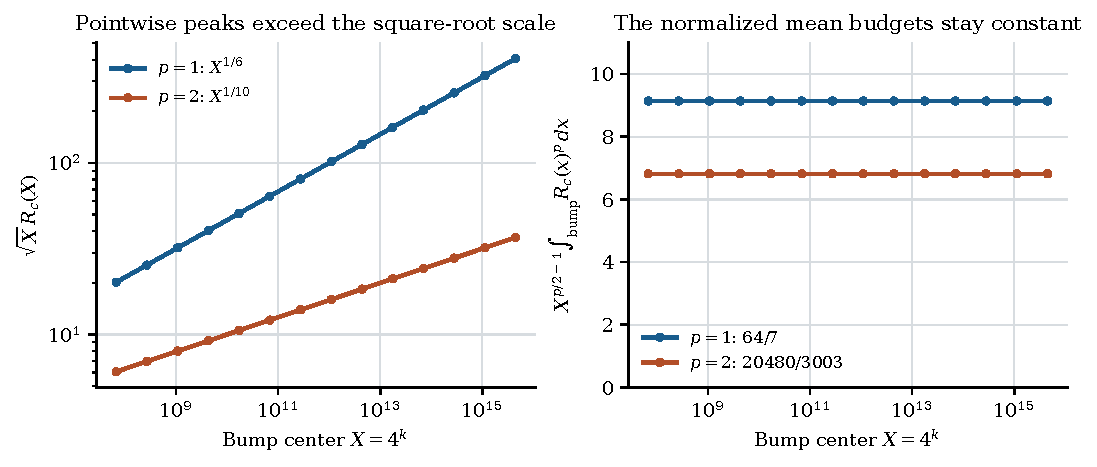
\includegraphics[width=\linewidth]{figures/mean_sharpness.pdf}
 \caption{The continuous sharpness models with $\gamma=1/2$.
 The normalized pointwise peaks grow, while their corresponding
 normalized moment budgets remain constant. Integer discretization
 changes the remainder by $O(1/x)$, preserving these asymptotics.
 These are synthetic positive weights, not prime data.}
 \label{fig:mpt-sharpness}
\end{figure}

The coefficients in Proposition~\ref{prop:mpt-sharp} satisfy a stronger
size bound than $a_n=O(\log n)$. They do not have prime-power support,
an Euler product, or an $L$-function functional equation. The example
therefore limits an abstract inference, without disproving any stronger
statement about actual primes.

\subsection{Compatibility with meromorphic continuation}

The countermodel also has the analytic properties relevant to the
mean criterion. This checks that the mean-to-pointwise gap is not
merely an artifact of a function lacking analytic continuation.

Write $(s)_j=s(s+1)\cdots(s+j-1)$, with $(s)_0=1$, and define
\[
 J_m(s)=\frac{(s)_{2m}}{(2m)!}
       \int_{-1}^1z^{2m}\psi(z)\,dz.
\]
Expanding $(1+\delta z)^{-s}$, where
$\delta=10X_k^{-\alpha/2}\le1/2$, and using the evenness of $\psi$
gives, initially far to the right,
\begin{equation}\label{eq:mpt-meromorphic}
 F_c(s)=\int_1^\infty R_c(x)x^{-s}\,dx
 =10\sum_{m\ge0}100^mJ_m(s)
 \frac{4^{k_0(1-s-\alpha(m+3/2))}}
      {1-4^{1-s-\alpha(m+3/2)}}.
\end{equation}
The series defines a meromorphic function on $\C$. Indeed, on any
compact set avoiding the displayed poles, its sufficiently late terms
are bounded by a polynomial in $m$ times
$(100\cdot4^{-k_0\alpha})^m$, and this geometric ratio is at most
$1/4$. Only finitely many remaining terms need separate consideration.
Possible poles are simple and lie at
\[
 s=1-\alpha(m+3/2)+\frac{2\pi i n}{\log4},
 \qquad m\ge0,\ n\in\mathbb Z.
\]
At a positive real pole $u=1-\alpha(m+3/2)$ the residue is
$10\cdot100^mJ_m(u)/\log4>0$. The rightmost line is
\[
 \Re s=1-3\alpha/2
 =1-\frac{3p\gamma}{2p+1}\le1-\gamma,
\]
with equality when $p=1$.
By \eqref{eq:mpt-discrete-error}, $F_d-F_c$ is holomorphic on
$\Re s>0$. Thus the discrete model has the same possible poles and
residues in that half-plane. Global meromorphic continuation of $F_d$
is not asserted.

At $\gamma=1/2$, these models satisfy the sharp mean budget and have
no pole to the right of $1/2$, yet their peaks decay only as
$x^{-p/(2p+1)}$. The usual sharper pointwise conclusions for arithmetic
$L$-functions require their additional structure and growth estimates.
For a proposed determinant transfer, the practical instruction is to
apply the mean criterion directly when it is available, while using
Theorem~\ref{thm:mpt-local} for finite-window or pointwise diagnostics.

\section{Which open questions are worth pursuing next?}

The review supports a focused research program. More character tables or more equivalent one-sided criteria would add less value than proving one new arithmetic estimate. The existing analytic interfaces already accept pointwise, sparse, averaged, and selected filtered forms of control.

\subsection{Highest priority: a fixed nonabelian field}

Two complementary benchmarks are useful. The earlier conductor-23 example has the simplest well-developed analytic target: if $H$ is the splitting field of $T^3-T-1$, its Dedekind zeta function contains a degree-two Hecke factor over $\Q(\sqrt{-23})$ that is not a Dirichlet factor over $\Q$. The new real discriminant-229 example is particularly suited to extending the internal CM-field construction, because its Galois closure is totally real and can be adjoined without destroying the CM structure.\cite{priorMean,Cogdell}

For the conductor-23 field, write
\[
 -\frac{\zeta_H'}{\zeta_H}(s)=\sum_{n\ge1}\frac{a_H(n)}{n^s},
 \qquad
 \zeta_H(s)=\frac{\kappa_H}{s-1}+\kappa_H\gamma_H+O(s-1).
\]
The positive coefficients satisfy $0\le a_H(n)\le6\Lambda(n)$. Define
\[
 R_H(x)=\sum_{n\le x}a_H(n)\left(\frac1n-\frac1x\right)
         -\log x+1+\gamma_H.
\]
Its Mellin transform is
\[
 -\frac{\zeta_H'(s)/\zeta_H(s)}{s(s-1)}
 -\frac1{(s-1)^2}+\frac{1+\gamma_H}{s-1}.
\]
The singularity at $s=1$ is removable. A zero $\rho$ of multiplicity $m_\rho$ gives residue $m_\rho/[\rho(1-\rho)]$, which is positive at real zeros in $(0,1)$. Therefore
\begin{equation}\label{eq:target-mean}
 \int_X^{2X}\pos{R_H(x)}\,dx\ll_\varepsilon X^{1/2+\varepsilon}
\end{equation}
would exclude zeros to the right of $1/2$ and the functional equation would finish RH for this field. A square moment $\ll_\varepsilon X^\varepsilon$ also suffices. These are established reductions in the earlier reports, included here to specify the actual remaining arithmetic objective.\cite{priorMean}

The two filtered bounds of Corollary~\ref{cor:joint-half} are an alternative target if direct-sum theta constructions naturally provide the combinations at $x,2x,4x$. The positive-ramp theorem explains their pointwise content, but no conversion to a pointwise square-root estimate is required before using Landau.

For the discriminant-229 construction, the next useful theorem is an odd-cocycle bound over the nonabelian CM tower with the right uniformity in the tower level and weight, or a globally admissible replacement for the source's two coprime integral frames. Either would remove a real obstruction. A proof of mere finiteness, with uncontrolled dependence on the growing parameters, is insufficient for the final scaling argument.

\subsection{A nearby arithmetic classification: exponent seven}

The validated exponent-six report also supplies an exact upper bound
\[
 |D|\le4\cdot4600^7
 =174\,327\,062\,886\,400\,000\,000\,000\,000
\]
for a possible omitted exponent-seven field. Its rational explicit-formula checks were rerun as part of the same script. EKN's initial range contains 33 such fields; the residual interval remains unexcluded here.\cite{EKN,priorSix}

The exponent-six collision works because the forced number of split primes exceeds the number of possible coefficients $b$ in the norm equation. At exponent seven the same parameter choices do not give that inequality. A successful extension needs a sharper split-prime test, a stronger restriction on the coefficients, or a multi-equation elimination. Reusing the sixth-power certificate with an exponent changed in the code would not prove completeness.

This is an attractive finite arithmetic problem, because its target and certificate format are concrete. It uses the availability of quadratic GRH together with new integral arithmetic, rather than requiring a nonabelian RH extension first.

\subsection{Other candidates and their actual status}

\begin{longtable}{@{}p{.22\textwidth}p{.35\textwidth}p{.36\textwidth}@{}}
\toprule
Target & Relevant idea & Missing substantive result\\
\midrule
\endhead
Hecke GRH over a fixed nontrivial field & Prime divisibility encoded by embeddings; one-sided residue barrier & A matched height/index/rank inequality for the new coefficients.\\[4pt]
Nonabelian Dedekind RH & Complete-splitting selectors; positive regular-character coefficients & The arithmetic estimate, plus auxiliary-twist control where the chosen statistic needs it.\\[4pt]
Artin holomorphy & Integral periods, congruences, determinant ratios & Holomorphy cannot be inferred from a generic zero-free estimate or weakened internal attachment notion.\\[4pt]
Selmer or $K$-group vanishing & Local twist selection; denominator and Fitting-ideal bounds & A precise comparison with the desired fixed module, controlled coefficient ramification, and a separating certificate.\\[4pt]
Sparse equations for singular moduli & Size-versus-integrality; conjugate-root and determinant constraints & After the prior five-term completion, new six-term or uniform support-growth arguments; old residual lists are superseded.\\[4pt]
Exponent-seven class-group census & Positive explicit-formula tests and norm collisions & Exclusion of the residual interval left by the validated upper bound.\\
\bottomrule
\end{longtable}

The prior sparse-CM reports contain additional arguments, not merely a quotation of Riffaut's known conditional result. This session checked selected exact Newton-disk, reduced-form and confluent-determinant inputs, but did not replay all of their global polynomial-identification and residue-sieve certificates. Those classifications are therefore catalogued with that narrower validation status; the exponent-six census is the arithmetic completion fully revalidated here.

\subsection{A practical stopping criterion for each transfer}

A transfer should be called a solved new zero problem only after all of the following mathematical steps have been supplied: a statistic with correct poles; integral or geometric objects that genuinely encode that statistic; upper and lower bounds for the same normalized covolume; a rank and denominator estimate in the required range; and the analytic implication with no hidden cancellation. The present report completes some reusable local and analytic steps and one independent arithmetic classification. It leaves the new nonabelian covolume estimate open.

\section{Verification, provenance, and reproduction}
\label{sec:reproduction}

\subsection{What was actually checked}

The readable upstream source was inspected at commit
\nolinkurl{72fead102f663d5c7a407964a13dc0cf9d977207}; the incoming reports were read at ProveIt commit
\nolinkurl{6fe2c1bd450aa7f19eab17fb9a6e76170b4fce00}. The archive inventory records all 26 ZIP files, their hashes, and the extracted text files. Selected upstream files are bundled with a manifest containing SHA-256 and Git-blob hashes. The source checker verifies those snapshots; it does not recompile the upstream project.

\begin{longtable}{@{}p{0.25\textwidth}p{0.67\textwidth}@{}}
\toprule
Component & Evidence and exact scope\\
\midrule
\endhead
Exponent-six exclusion & Mathematical proof review; rational explicit-formula enclosures; complete Python and C++ paired-norm searches, each testing 9,393,302 relevant values and finding zero survivors.\\[4pt]
Field and order lists & Distinctness, counts, largest discriminants, original order-table Git blob, and exact matching of the 432 fundamental entries. The published initial field census and the conductor classification are inputs.\\[4pt]
Nonabelian local frame & Exact trace matrices, Gram diagonalization, frame weights, compatible-embedding and finite-group identities, and two explicit prime examples. General statements also have written proofs in Section~\ref{sec:nonabelian-frame}.\\[4pt]
Joint filters & Written Mellin/Landau proof; exact polynomial and reconstruction identities; a counterexample explaining individual-filter blindness.\\[4pt]
Positive-ramp moments & Written proof, exact rational derivative and bump-area checks, a discrete bounded-coefficient example, and a separate independent review of all constants and continuation statements.\\[4pt]
Elementary Lean components & Seven lemmas compiled with Lean 4.35.0 and Mathlib \texttt{56a005855ea17e0b0958f73ec801ae140b0a1679}. The printed dependency lists contain only standard axioms.\\[4pt]
Other incoming claims & Claim-by-claim inventory and overlap review. Selected sparse-CM inputs were independently checked; the complete large CM sieves were not replayed.\\
\bottomrule
\end{longtable}

The seven Lean lemmas concern the polynomial B\'ezout identity, absence of a common filter zero, pointwise filter reconstruction, convexity of one hinge, its weighted version, finite positive-ramp convexity, and algebraic cancellation in a rank/covolume inequality. They certify useful exact pieces. They do not formalize the analytic continuation theorem, the complete moment theorem, the class-group census, or a new RH assertion. The file contains no \texttt{sorry} or additional axioms.

\subsection{How to reproduce the package}

From the extracted archive root, run
\begin{verbatim}
python3 code/reproduce.py
python3 code/reproduce.py --full-census
python3 code/build_pdf.py
\end{verbatim}
The first command reruns the short exact certificates. The second also compiles and executes the two complete residual-interval searches and the rational test, comparing their deterministic results with the delivered logs. Python~3, SymPy, and a C++17 compiler are needed for the complete arithmetic replay. Matplotlib is needed only to regenerate the illustrative figure. The PDF requires a LaTeX installation with the packages listed in \texttt{report.tex}; the build helper includes a fallback for incomplete TeX path configuration.

For the separate Lean file, with \texttt{elan}/\texttt{lake} installed and network access to the pinned dependencies, run
\begin{verbatim}
cd formalization
lake update
lake exe cache get
lake env lean TransferCore.lean
\end{verbatim}
Alternatively, \texttt{code/reproduce.py --lean} runs the compilation in the supplied formalization project after its dependencies have been prepared. The delivered log records this session's actual successful compilation. Dependency caches and compiled Lean objects are not bundled.

The fresh replay workspace is kept under \texttt{validation/replay/}; it does not overwrite the supplied certificates. The earlier exponent-six programs and tables are retained unchanged under \texttt{prior/exponent\_six/}. Their origin and unchanged-file comparisons are recorded separately from the new checkers. The root \texttt{SHA256SUMS} covers the final package's files, excluding itself.

\subsection{Limits that matter mathematically}

The exponent-six proof still depends on the correctness of EKN's published exhaustive census through $3.1\cdot10^{20}$ and the cited conductor theorem. The exact searches here close the residual interval; they are not a recomputation of every class group in the original census. Likewise, the source snapshots and external kernel-check reports should not be confused with a fresh full rebuild by this investigation.

The frame and averaging results are proved mathematical interfaces. Their usefulness for a new zero problem depends on a missing global arithmetic estimate, identified explicitly in Sections~\ref{sec:nonabelian-frame} and~\ref{sec:joint-filters}. No new nonabelian RH, general Artin holomorphy, Vandiver assertion, Bloch--Kato assertion, or fixed algebraic $K$-group vanishing theorem is claimed.

The comparison with prior reports is relative to the supplied 26-archive corpus and the cited primary literature. It establishes what was reused and what was added in this synthesis; it does not establish worldwide priority for the elementary analytic or trace-form ingredients.

\appendix
\section{The 26 incoming reports: reuse and claim status}

This index records the inspected corpus at the pinned ProveIt commit. ``Written result'' means that a report supplies a mathematical argument; it is not a blanket certification of every assertion. ``Reduction'' means the new zero theorem still depends on an unproved arithmetic estimate. The accompanying CSV and JSON retain fuller descriptions, cautions, archive hashes, and source locations.

The principal overlap decisions are these. The exponent-six completion below supersedes earlier partial exclusions. The sparse-CM completion claims to close the five exceptional all-width cases left by earlier reports; only selected exact inputs were replayed here. Fourth-power sampling, positive-part Mellin control, torsion-grid selection, and general finite-group detectors are already in the corpus. They are used as a baseline rather than relabelled as new results.

\small
\begin{longtable}{@{}r p{0.38\textwidth} p{0.53\textwidth}@{}}
\toprule
ID & Archive & Main content and status in this investigation\\
\midrule
\endhead
00 & \path{dirichlet-grh-research.zip} & O'Hara finiteness, heavenly varieties, moving-height Euler products, and rational-ratio spectra. Prior written arguments; extensive arithmetic not replayed here.\\[5pt]
01 & \path{grh-arithmetic-transfers.zip} & Prime-plus-cube and isogeny applications; nonabelian one-sided criterion. Prior written deductions; local surviving candidates do not prove existence.\\[5pt]
02 & \path{grh-exponent-six-and-transfers.zip} & \textbf{Revalidated completion: 432 fields and 1,236 orders of exponent six.} Full residual-interval tests replayed; initial published census remains an input.\\[5pt]
03 & \path{grh-lean-transfers.zip} & CM, genus, reflection, and prime-race deductions. Read with later completions; earlier residual lists are not the current state.\\[5pt]
04 & \path{grh-transfer.zip} & Abelian Mertens-error census, norm-Euclidean transfers, representation questions, Kummer criterion. New Kummer estimate remains open.\\[5pt]
05 & \path{grh_a6_transfer_2026-11-25.zip} & $A_6$ entire detectors, degree bounds, and dyadic equivalences. Group/analytic reductions; new prime bound missing.\\[5pt]
06 & \path{grh_beyond_dirichlet_grh_2026-11-25.zip} & Common torsion nonvanishing, formal series, determinant/Fitting approximation, odd-cocycle comparison. Selected proofs reviewed; no new named conjecture resolved.\\[5pt]
07 & \path{grh_cm_four_terms_and_prime_bias.zip} & Four-term CM classification, almost-complete quintic cases, Suzuki signs, simultaneous balance. CM residuals superseded by 20; central nonvanishing not proved.\\[5pt]
08 & \path{grh_cm_prime_applications.zip} & Initial sparse-CM reductions, prime-generating constants, prime-plus-powers, sparse scales. Already includes fourth-power sampling and credits its antecedent.\\[5pt]
09 & \path{grh_cm_sparse_equations.zip} & Four-term classification and five exceptional five-term cases; support growth. The all-width exceptional cases are treated later in 20.\\[5pt]
10 & \path{grh_cyclic_generator_transfer_2026-11-25.zip} & Cyclic-generator detector refinement, explicit $S_8$ weights, Gamma averaging, simultaneous convexification. Arithmetic comparison missing.\\[5pt]
11 & \path{grh_deficit_transfer_2026-11-25.zip} & Optimal nonnegative Frobenius deficits, constant-removing differences, averaged positive part. New nonabelian and automorphic inequalities remain unproved.\\[5pt]
12 & \path{grh_kummer_window_transfer_2026-11-25.zip} & Kummer positive-block criterion and primitive-root density reduction; multiple tests in short windows. Arithmetic-geometric inequality missing.\\[5pt]
13 & \path{grh_lean_transfer_analysis.zip} & Source audit, abstract covolume/rank transfer, sparse auxiliary primes, conductor-23 target. New arithmetic and twist inputs missing.\\[5pt]
14 & \path{grh_method_transfers_2026-11-25 (2).zip} & \textbf{Reused analytic baseline:} positive-part Mellin, dyadic moments, moving-box obstruction, inverse-rank loss. $K$-theory screening is not a vanishing theorem.\\[5pt]
15 & \path{grh_method_transfers_2026-11-25(1).zip} & Infinite-family torsion selector, degree-independent grid, $A_5$ detector, partial exponent-six exclusions. Selector extension already exists; census superseded by 02.\\[5pt]
16 & \path{grh_method_transfers_2026-11-25.zip} & \textbf{Reused geometric baseline:} reciprocal convexity, fourth-power sampling and sharpness, periodic obstruction, root counts, ramification budgets. These are not new here.\\[5pt]
17 & \path{grh_quantitative_twists_2026-11-25.zip} & Fixed-packet polynomial twist bounds, admissible shells, bounded-series and determinant variants. Fixed witness-radius comparison is weaker than the source's selected-radius comparison.\\[5pt]
18 & \path{grh_reflection_transfer_2026-11-25.zip} & $S_n$ and reflection-group zero-multiplicity inequalities and two-class prime criterion. Prime estimate missing.\\[5pt]
19 & \path{grh_relative_prime_races_2026-11-25.zip} & Entire relative factors in normal towers; cancellation of intermediate strata; $S_4$ weights. New analytic inequality missing.\\[5pt]
20 & \path{grh_sparse_singular_moduli.zip} & Claims global $s\le5$ iff $h\le4$, support growth, exact families, and a $D_4$ criterion. Here: 18 disk, 245 reduced-form, and 17 period inputs checked; large global sieve not replayed.\\[5pt]
21 & \path{grh_sylow_transfer_2026-11-25.zip} & Commutator-Sylow statistics, Heilbronn multiplicity control, $\operatorname{PSL}_2(7)$ weights. Arithmetic estimate missing; later refinement in 10.\\[5pt]
22 & \path{grh_transfer_analysis.zip} & Source audit, standard consequences, abstract analytic extraction, conductor-23 target, elementary Lean lemmas. Small Lean file does not establish target arithmetic.\\[5pt]
23 & \path{grh_transfer_analysis_2026-11-25.zip} & Standard consequences, one-sided criterion, auxiliary-prime families, $S_3$ tensor-square target. Arithmetic/twist estimate missing; wrappers explicitly uncompiled.\\[5pt]
24 & \path{grh_transfers.zip} & Partial exponent-six completion, modulo-four race, cubic-$23$ eventual sign. Census superseded by 02; cubic sign estimate remains open.\\[5pt]
25 & \path{psl2_grh_transfer.zip} & $\operatorname{PSL}_2(2^r)$ detector optimality and root-count equivalence. Finite group checks support the group claims; the prime inequality remains open.\\
\bottomrule
\end{longtable}
\normalsize

The inventory's extracted-file paths describe the analysis workspace, not a promise that every earlier archive is duplicated in this ZIP. The selected certificates needed to reproduce this report are included; the complete older archives remain available at the pinned repository link in~\cite{priorCollection}.

\begin{thebibliography}{99}
\addcontentsline{toc}{section}{References}

\bibitem{source}
Luke Sernau and contributors,
\emph{grh-lean: a shortened Lean proof of RH and Dirichlet GRH},
25 November 2026, commit
\texttt{72fead102f663d5c7a407964a13dc0cf9d977207}.
\url{https://github.com/lsernau/grh-lean/tree/72fead102f663d5c7a407964a13dc0cf9d977207}.
Source guide and individual declaration links are given in the text.

\bibitem{Sutherland}
Andrew Sutherland,
\emph{Verification files for the shorter Lean proof of RH and GRH},
status page accessed 25 November 2026 (Pacific time).
\url{https://math.mit.edu/~drew/shortgrh/}.
Checks are external evidence, not checks performed by this report.

\bibitem{Rubinstein}
Michael Rubinstein,
\emph{An independent check of the short Lean proof of RH and GRH},
status page accessed 25 November 2026 (Pacific time).
\url{https://mrubinst.github.io/grh-lean-compact-check/}.

\bibitem{priorCollection}
Vladimir Reshetnikov, ProveIt repository, \emph{docs/incoming},
commit \texttt{6fe2c1bd450aa7f19eab17fb9a6e76170b4fce00}.
The 26 supplied archives are indexed in Appendix~A and in
\texttt{evidence/prior\_claim\_status.csv}.
\url{https://github.com/VladimirReshetnikov/ProveIt/tree/6fe2c1bd450aa7f19eab17fb9a6e76170b4fce00/docs/incoming}.
These are prior research reports supplied for analysis; the repository location is not an assertion of journal publication or authorship of every archive.

\bibitem{priorSix}
Prior ProveIt report,
\emph{grh-exponent-six-and-transfers.zip},
in~\cite{priorCollection}; especially \texttt{global-bound.tex},
\texttt{local.tex}, and the rational and paired-norm certificates.
Unchanged relevant code and data, with fresh replay logs, are supplied here under
\texttt{prior/exponent\_six/}.

\bibitem{priorMean}
Prior ProveIt report,
\emph{grh\_method\_transfers\_2026-11-25 (2).zip},
in~\cite{priorCollection}.
Positive-part Mellin criterion, dyadic moment conditions, moving-box multiplier obstruction, and rank/index/denominator loss criterion.

\bibitem{priorSampling}
Prior ProveIt report,
\emph{grh\_method\_transfers\_2026-11-25.zip},
in~\cite{priorCollection}.
Reciprocal-variable convexity, sparse sampling, fourth-power checkpoints, periodic Frobenius obstruction, and ramification budget.

\bibitem{EKN}
Andreas-Stephan Elsenhans, J\"urgen Kl\"uners, and Florin Nicolae,
\emph{Imaginary quadratic number fields with class groups of small exponent},
arXiv:1803.02056 (2018).
Theorem~1 and Table~1: the initial exhaustive census;
Theorem~3 and Table~2: ERH discriminant bounds;
Theorem~2 excludes exponents six and seven from its completeness assertion.
\url{https://arxiv.org/abs/1803.02056}.

\bibitem{ARSX}
David Aiken, Erick Ross, Dmitriy Shvydkoy, and Hui Xue,
\emph{Boundary CM points and class groups of small exponent},
arXiv:2605.26020v1 (25 May 2026).
Theorem~1.3(5) and its conductor analysis supply the order classification subject to the remaining fundamental-discriminant interval.
\url{https://arxiv.org/html/2605.26020v1}.

\bibitem{orderData}
Erick Ross, research data accompanying~\cite{ARSX},
\emph{class-groups-small-exp/Table-6.txt},
commit \texttt{119301b8bcae42a891062d4877b77b6dbc8e820f}.
\url{https://github.com/erick-ross/research-data/blob/119301b8bcae42a891062d4877b77b6dbc8e820f/class-groups-small-exp/Table-6.txt}.
The exact Git blob checked here is
\texttt{fc8d109c749eb73efab6bc5d9f058c5c78cd8c8f}.

\bibitem{Carneiro}
Emanuel Carneiro, Micah B. Milinovich, Emily Quesada-Herrera, and Antonio Pedro Ramos,
\emph{Fourier optimization, the least quadratic non-residue, and the least prime in an arithmetic progression},
arXiv:2404.08380v2 (12 August 2025), Lemma~9.
\url{https://arxiv.org/abs/2404.08380}.

\bibitem{Suzuki}
Masatoshi Suzuki,
\emph{On variants of Chebyshev's conjecture},
The Ramanujan Journal \textbf{68}, article 95 (2025),
arXiv:2411.07436v3.
\url{https://doi.org/10.1007/s11139-025-01238-9}.

\bibitem{Setiawan}
Sandi Setiawan,
\emph{The Primacohedron Trace Formulation of the Riemann Hypothesis: A Guide to Reconstructing the Alp\"oge--Claude Proof in Lean},
Preprints.org, 202611.0738v2 (25 November 2026).
\url{https://www.preprints.org/manuscript/202611.0738/v2}.
Unrefereed preprint, cited for an antecedent of fourth-power sampling credited in the supplied reports, not used as an unproved input to the new theorems.

\bibitem{BFM}
J. Ederson M. Braga, Alessio Figalli, and Diego Moreira,
\emph{Optimal regularity for the convex envelope and semiconvex functions related to supersolutions of fully nonlinear elliptic equations},
Communications in Mathematical Physics (2019), Section~8, Proposition~8.2.
\url{https://cvgmt.sns.it/media/doc/paper/4316/CMP-CE-BFM.pdf}.

\bibitem{Cogdell}
James W. Cogdell,
\emph{On Artin $L$-functions}, author-hosted survey.
\url{https://people.math.osu.edu/cogdell.1/artin-www.pdf}.
Used for the distinction between Dirichlet, Hecke, and Artin factorizations.

\end{thebibliography}

\end{document}
